\section{Edycja danych}

Po zapisaniu najnowszych danych, następnym krokiem jest wprowadzenie niezbędnych aktualizacji dotyczących usług. W związku z tym utworzono dwa ekrany -- pierwszy służy do wyboru usługi z listy, a drugi przedstawia niezbędne szczegóły oraz umożliwia edycję związanych z nią informacji.

\subsection{Ekran wyboru usługi do edycji}

\begin{figure}[h]
    \centering
    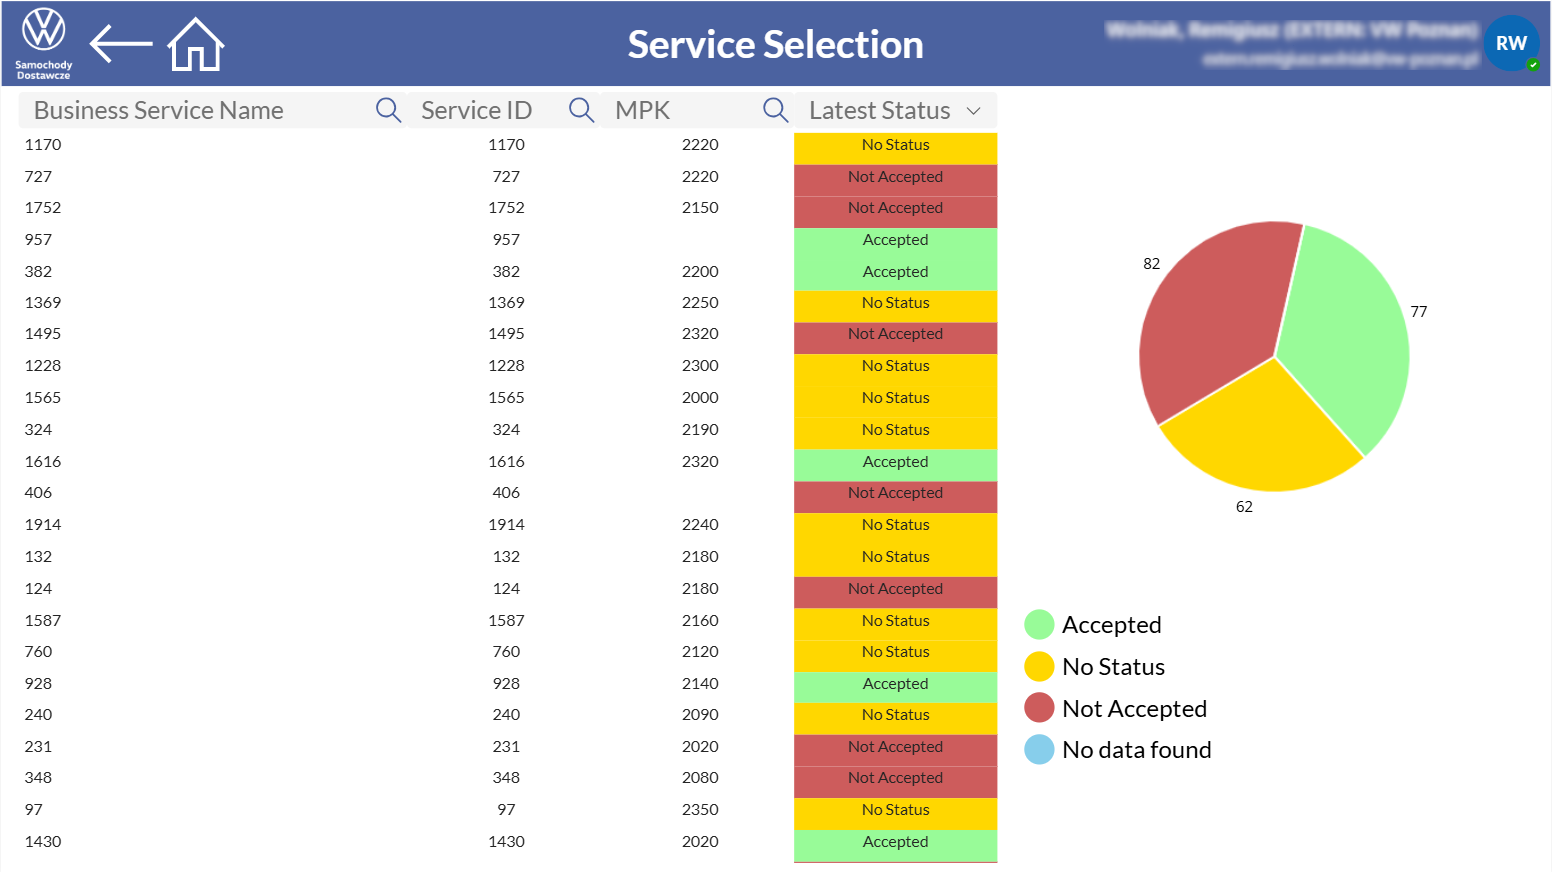
\includegraphics[width=0.9\textwidth]{figures/ServiceSelectionForm.png}
    \caption{Ekran wyboru usługi do edycji}  
    \label{fig:ServiceSelectionForm}
\end{figure}

\begin{comment}

Ekran wyboru elementu do obróbki składa się z: \begin{enumerate}
    \item listy, przedstawiającej dane z tymczasowej kolekcji \textit{MergedData}, utworzonej specjalnie na potrzeby obsługi wyboru danych do edycji,
    \item pól wyszukiwania i filtrów, umożliwiających zawężenie listy na podstawie nazwy usługi, identyfikatora (\textit{Service ID}), miejsca powstawania kosztów (\textit{MPK}) oraz statusu decyzji (\textit{Accepted}, \textit{Not Accepted}, \textit{No Status}),
    \item wykresu kołowego, prezentującego wizualne podsumowanie liczby elementów w każdej kategorii statusu decyzji,
    \item interfejsu umożliwiającego dynamiczne dopasowanie wyników listy w czasie rzeczywistym, na podstawie wprowadzonych kryteriów wyszukiwania,
    \item nagłówka, który przedstawia kontekst użytkownika, w tym nazwę i dane aktualnie zalogowanego użytkownika. \end{enumerate}
\end{comment}

\subsubsection*{Lista wyboru serwisu}
Lista prezentuje dane pochodzące z dynamicznej kolekcji \textit{MergedData}, która została utworzona w celu zintegrowania informacji z trzech różnych list SharePoint (\textit{Lista\_Uslug}, \textit{Lista\_Kwot}, \textit{Lista\_Indykacji}). Dzięki zastosowaniu wbudowanych funkcji \textit{LookUp} (wyszukiwanie pojedynczego elementu w źródle danych na podstawie warunku) oraz \textit{AddColumns} (dodawanie nowych kolumn do istniejącego źródła danych), dane są filtrowane tak, aby wyświetlać jedynie najnowsze rekordy, np. dla najświeższych decyzji i kwot. Taka struktura zapewnia użytkownikom dostęp do aktualnych informacji bez konieczności ręcznego przeszukiwania źródłowych list. Lista jest dynamiczna, co oznacza, że zmiany w danych źródłowych są automatycznie uwzględniane.

Każdy element na liście posiada dodatkową funkcję interakcji. Po najechaniu kursorem na wybraną usługę (funkcja \textit{hover}), element wizualnie zmienia swój wygląd -- zwęża się, zmienia kolor oraz staje się możliwy do kliknięcia. Kliknięcie przenosi użytkownika do dedykowanego ekranu edycji, który umożliwia szczegółowe zarządzanie wybraną usługą.

\subsubsection*{Pola wyszukiwania i filtry}
Użytkownik ma możliwość zawężenia widocznych danych poprzez zastosowanie różnych kryteriów wyszukiwania. Pola obejmują:
\begin{itemize}
    \item {Wyszukiwanie po nazwie usługi (\textit{Service Name})} -- Obsługuje częściowe dopasowania dzięki wbudowanej funkcji \textit{StartsWith} (sprawdza, czy ciąg tekstowy zaczyna się od określonej frazy).
    \item {Filtrowanie po identyfikatorze usługi (\textit{Service ID})} -- Umożliwia precyzyjne wyszukiwanie konkretnego elementu.
    \item {Filtrowanie według miejsca powstawania kosztów (\textit{MPK})} -- Pozwala na szybkie odnalezienie danych przypisanych do konkretnego obszaru finansowego.
    \item {Filtrowanie według statusu decyzji (\textit{Accepted}, \textit{Not Accepted}, \textit{No Status})} -- Dzięki zastosowaniu funkcji \textit{Switch} (zwraca wartość w zależności od spełnionego warunku), wartości statusów są mapowane na odpowiednie kody liczbowe.
\end{itemize}
Filtry te mogą być stosowane jednocześnie, co umożliwia precyzyjne dopasowanie wyświetlanych danych.

\subsubsection*{Wykres kołowy}
Wykres kołowy ilustruje podział danych według statusów decyzji. Każdy segment odpowiada liczbie elementów z przypisanym statusem, co pozwala użytkownikowi szybko ocenić proporcje między kategoriami (\textit{Accepted}, \textit{Not Accepted}, \textit{No Status}). Wykres jest dynamiczny -- aktualizuje się w czasie rzeczywistym w oparciu o zastosowane filtry.



\subsection{Ekran edycji elementu}
Ekran edycji elementu, widoczny na rysunku \ref{fig:EditForm}, prezentuje szczegółowe informacje dotyczące wybranej usługi, umożliwiając analizę danych historycznych oraz wprowadzanie nowych decyzji. Ekran składa się z kilku logicznie ułożonych sekcji, które są opisane poniżej.
\begin{figure}[h]
    \centering
    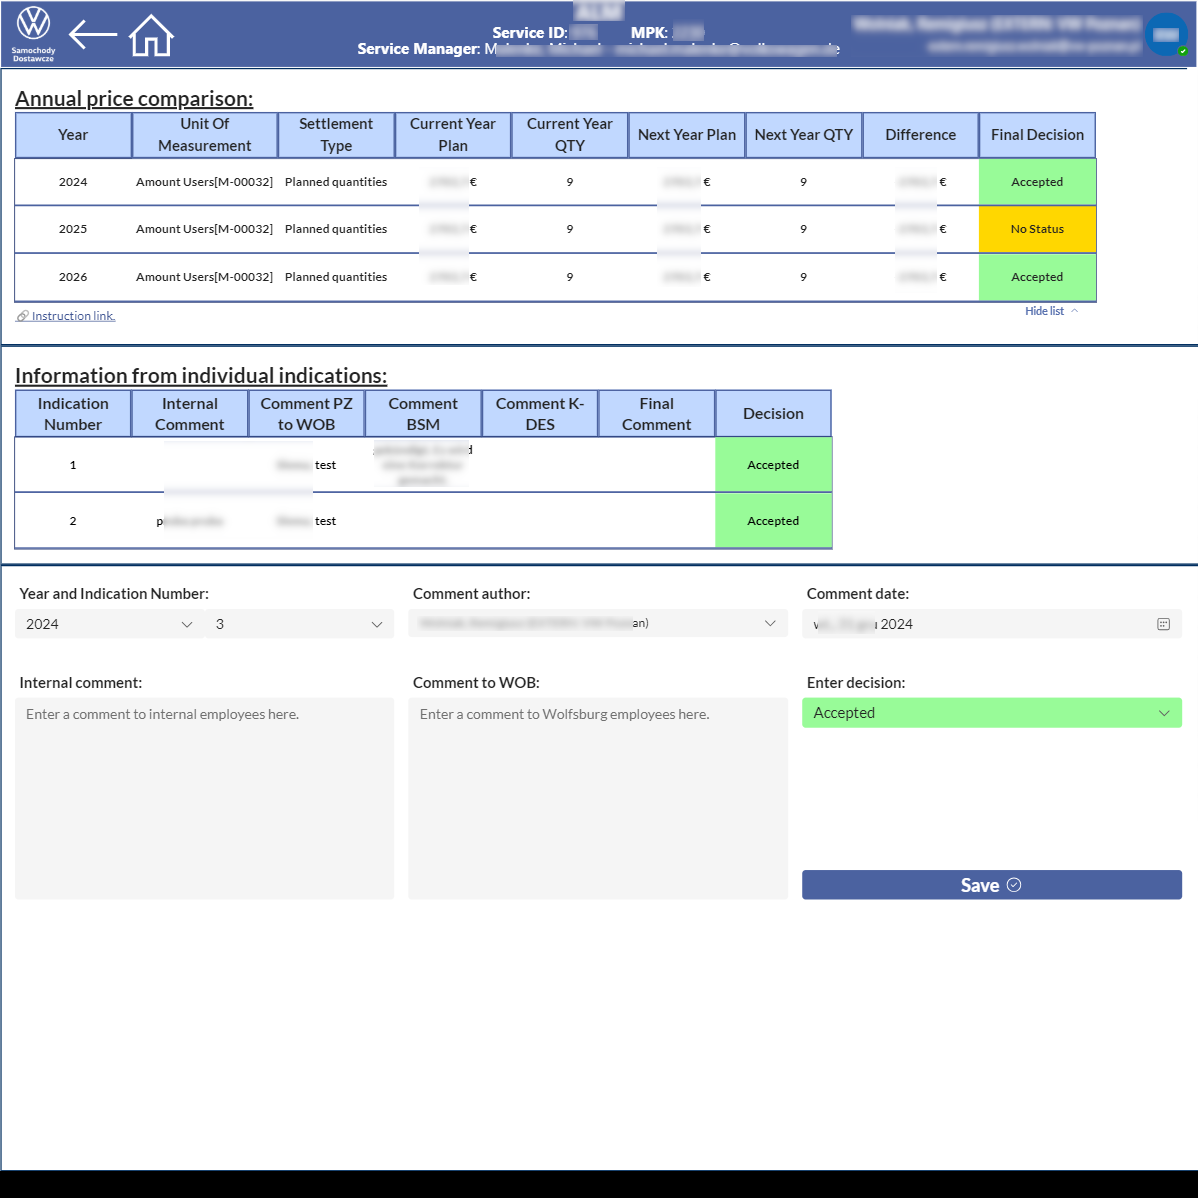
\includegraphics[width=0.9\textwidth]{figures/EditForm.png}
    \caption{Ekran edycji elementu}  
    \label{fig:EditForm}
\end{figure}
\subsubsection{Porównanie finalnych decyzji z poprzednich lat}
W górnej części ekranu znajduje się tabela przedstawiająca porównanie danych finansowych oraz decyzji z trzech ostatnich lat. Dane te są automatycznie pobierane i zawierają:
\begin{itemize}
    \item {Rok (Year)} -- okres, którego dotyczy dana decyzja,
    \item {Jednostka miary (Unit Of Measurement)} -- zazwyczaj ilość licencji. \customnote{w sumie to czasem było niecałkowite to idk}
    \item {Zeszłoroczne i planowane na następny rok wartości finansowe} -- np. \textit{Current Year Plan} oraz \textit{Next Year Plan},
    \item {Różnice w finansach (Difference)} -- różnica między zeszłorocznymi i potencjalnymi przyszłymi kosztami,
    \item {Status końcowej decyzji (Final Decision)} -- decyzje dotyczące planów z danego roku (\textit{Accepted, Not Accepted, No Status}).
\end{itemize}

Sekcja ta pozwala użytkownikowi przeanalizować ostatnie decyzje oraz ocenić trendy finansowe dla danej usługi w kolejnych latach.

\subsubsection{Link do instrukcji obsługi}
Poniżej tabeli z porównaniem decyzji znajduje się link do dedykowanej instrukcji obsługi usługi. Za pomocą linku użytkownik posiada dostęp do szczegółowych informacji na temat zasad korzystania z danej usługi, co może być przydatne podczas edycji danych lub wprowadzania nowych decyzji.

\subsubsection{Porównanie tegorocznych indykacji}
Sekcja ta prezentuje szczegóły kolejnych indykacji w ramach bieżącego roku. Użytkownik może zobaczyć i analizować szczegóły poszczególnych indykacji, takich jak:
\begin{itemize}
    \item {Numer indykacji (Indication Number)} -- \customnote{\textbf{??? wtf ->} numer kolejny przypisany do konkretnej decyzji},
    \item {Komentarze} -- w tym \textit{Internal Comment, Comment PZ to WOB, Comment K-DES}, które umożliwiają przekazanie informacji pomiędzy działami,
    \item {Data i autor komentarza} -- \customnote{\textbf{tutaj umo też zbędne bo chyba nie trzeba tłumaczyć że autor komentarza to autor komentarza a data komentarza to data komentarza nie?} dane dotyczące daty wprowadzenia decyzji oraz osoby odpowiedzialnej},
    \item {Status decyzji (Decision)} -- użytkownik może zobaczyć, czy decyzja została zaakceptowana (\textit{Accepted}), odrzucona (\textit{Not Accepted}) lub jeszcze nie podjęta (\textit{No Status}).
\end{itemize}

\subsubsection{Formularz do uzupełnienia danych}
Na samym dole strony znajduje się formularz umożliwiający wprowadzenie nowych danych lub aktualizację istniejących rekordów. Formularz zawiera pola takie jak:
\begin{itemize}
    \item {Rok (\textit{Year})} -- użytkownik może wybrać rok, którego dotyczy wpis,
    \item {Numer indykacji (\textit{Indication Number})} -- kolejny numer przypisany do decyzji,
    \item {Komentarze} -- pola do wprowadzenia uwag wewnętrznych, komentarzy między działami oraz końcowych komentarzy,
    \item {Status decyzji (\textit{Decision})} -- lista rozwijana, umożliwiająca wybór odpowiedniego statusu (\textit{Accepted, Not Accepted, No Status}),
    \item {Data i autor} -- data oraz osoba odpowiedzialna za wprowadzenie wpisu.
\end{itemize}

Przycisk \textit{Save} umożliwia zapisanie wprowadzonych zmian. Mechanizm ten:
\begin{itemize}
    \item Sprawdza istnienie wcześniejszych indykacji, aby upewnić się, że zachowana jest poprawna kolejność numeracji,
    \item W przypadku istniejącego wpisu -- aktualizuje dane (\textit{Patch}),
    \item W przypadku nowego wpisu -- tworzy nowy rekord (\textit{Defaults}),
    \item Resetuje pola formularza oraz odświeża dane na ekranie, aby uwzględnić ostatnie zmiany,
    \item Informuje użytkownika o powodzeniu lub błędach operacji za pomocą komunikatów (\textit{Notify}).
\end{itemize}

\subsubsection{Podsumowanie}
\customnote{\textbf{To to chyba do rozdziału 'Podsumowanie' bedzie co?}
    Ekran edycji elementu został zaprojektowany tak, aby umożliwić użytkownikom zarówno przeglądanie historycznych danych finansowych, jak i łatwe wprowadzanie nowych decyzji lub modyfikację istniejących. Dzięki logicznemu układowi sekcji oraz dynamicznej aktualizacji danych, interfejs wspiera efektywne zarządzanie informacjami dla każdej usługi.}
